\documentclass{standalone}
\usepackage{tikz}
\usetikzlibrary{patterns, positioning}

\begin{document}
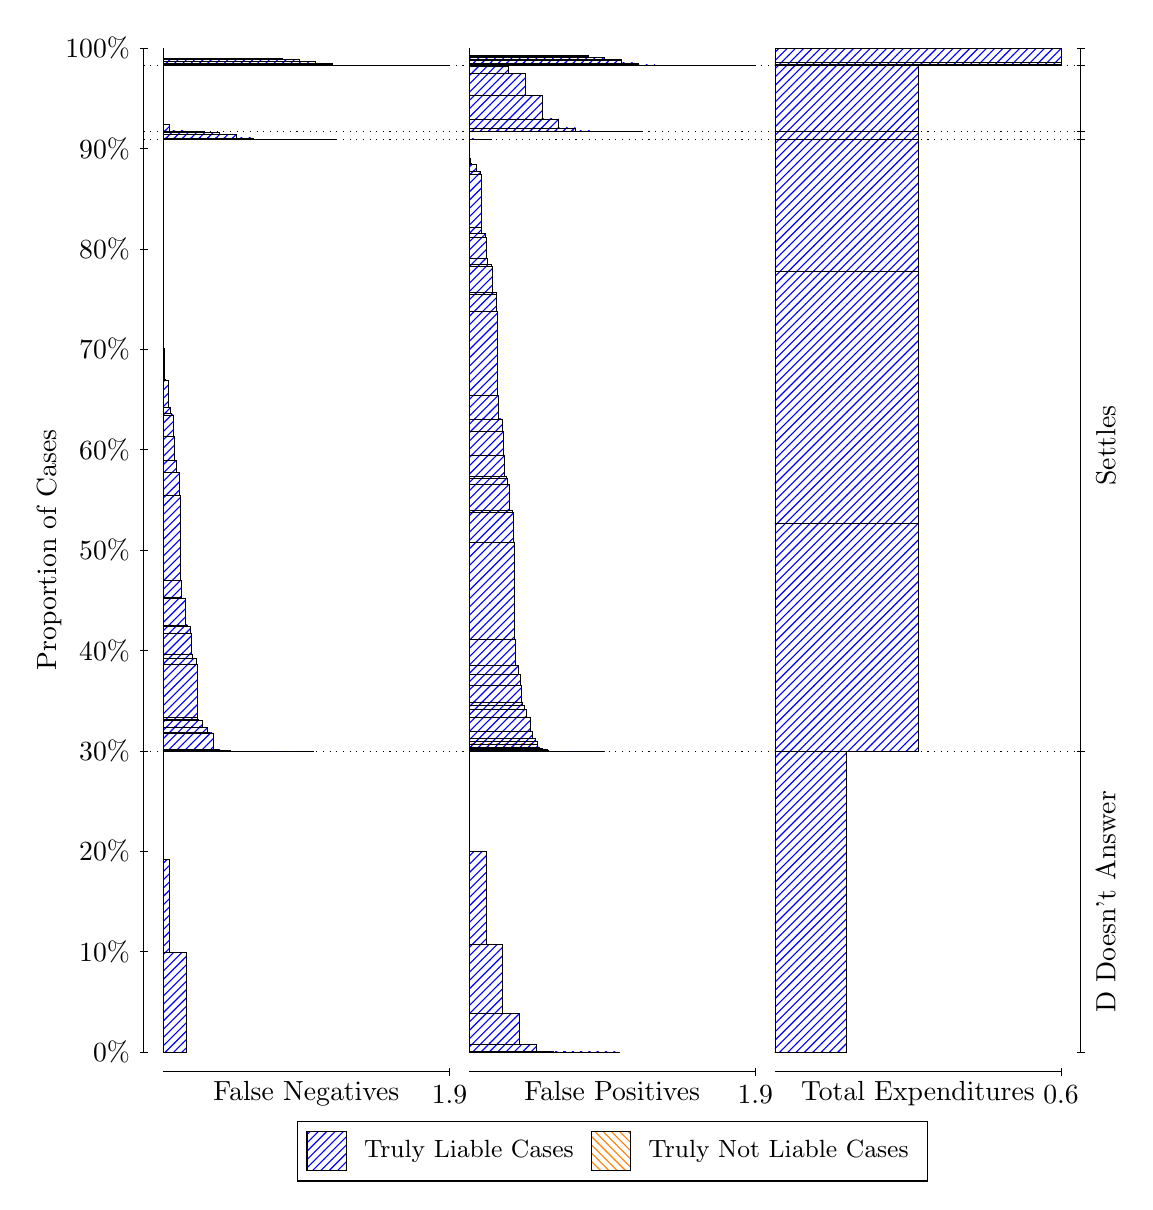
\begin{tikzpicture}
\draw[black, very thin] (1.5,1.75) -- (1.5,14.5);
\node[rotate=90, anchor=center] at (0.3, 8.125) {Proportion of Cases};
\draw[black, very thin] (1.45,1.75) -- (1.55,1.75);
\node[anchor=east] at (1.45, 1.75) {0\%};
\draw[black, very thin] (1.45,3.025) -- (1.55,3.025);
\node[anchor=east] at (1.45, 3.025) {10\%};
\draw[black, very thin] (1.45,4.3) -- (1.55,4.3);
\node[anchor=east] at (1.45, 4.3) {20\%};
\draw[black, very thin] (1.45,5.575) -- (1.55,5.575);
\node[anchor=east] at (1.45, 5.575) {30\%};
\draw[black, very thin] (1.45,6.85) -- (1.55,6.85);
\node[anchor=east] at (1.45, 6.85) {40\%};
\draw[black, very thin] (1.45,8.125) -- (1.55,8.125);
\node[anchor=east] at (1.45, 8.125) {50\%};
\draw[black, very thin] (1.45,9.4) -- (1.55,9.4);
\node[anchor=east] at (1.45, 9.4) {60\%};
\draw[black, very thin] (1.45,10.675) -- (1.55,10.675);
\node[anchor=east] at (1.45, 10.675) {70\%};
\draw[black, very thin] (1.45,11.95) -- (1.55,11.95);
\node[anchor=east] at (1.45, 11.95) {80\%};
\draw[black, very thin] (1.45,13.225) -- (1.55,13.225);
\node[anchor=east] at (1.45, 13.225) {90\%};
\draw[black, very thin] (1.45,14.5) -- (1.55,14.5);
\node[anchor=east] at (1.45, 14.5) {100\%};

\draw[black, very thin] (13.4,1.75) -- (13.4,14.5);
\draw[black, very thin] (13.35,1.75) -- (13.45,1.75);
\node[anchor=west] at (13.35, 1.75) {};
\draw[black, very thin] (13.35,5.5631) -- (13.45,5.5631);
\node[anchor=west] at (13.35, 5.5631) {};
\draw[black, very thin] (13.35,13.34) -- (13.45,13.34);
\node[anchor=west] at (13.35, 13.34) {};
\draw[black, very thin] (13.35,13.437) -- (13.45,13.437);
\node[anchor=west] at (13.35, 13.437) {};
\draw[black, very thin] (13.35,14.275) -- (13.45,14.275);
\node[anchor=west] at (13.35, 14.275) {};
\draw[black, very thin] (13.35,14.5) -- (13.45,14.5);
\node[anchor=west] at (13.35, 14.5) {};

\draw[black, very thin, pattern color=blue, pattern=north east lines] (1.75,1.75) rectangle (2.0368,3.0136);
\draw[black, very thin, pattern color=blue, pattern=north east lines] (1.75,3.0136) rectangle (1.8244,4.1973);
\draw[black, very thin, pattern color=orange, pattern=north west lines] (1.75,4.1973) rectangle (1.75,4.1973);
\draw[black, very thin, pattern color=blue, pattern=north east lines] (1.75,4.1973) rectangle (1.75,5.5631);
\draw[black, very thin, pattern color=blue, pattern=north east lines] (1.75,5.5631) rectangle (3.6623,5.5631);
\draw[black, very thin, pattern color=blue, pattern=north east lines] (1.75,5.5631) rectangle (3.4711,5.5631);
\draw[black, very thin, pattern color=blue, pattern=north east lines] (1.75,5.5631) rectangle (3.4498,5.5631);
\draw[black, very thin, pattern color=blue, pattern=north east lines] (1.75,5.5631) rectangle (3.3754,5.5631);
\draw[black, very thin, pattern color=blue, pattern=north east lines] (1.75,5.5631) rectangle (3.2586,5.5631);
\draw[black, very thin, pattern color=blue, pattern=north east lines] (1.75,5.5631) rectangle (3.2373,5.5631);
\draw[black, very thin, pattern color=blue, pattern=north east lines] (1.75,5.5631) rectangle (3.1842,5.5631);
\draw[black, very thin, pattern color=blue, pattern=north east lines] (1.75,5.5631) rectangle (3.163,5.5631);
\draw[black, very thin, pattern color=blue, pattern=north east lines] (1.75,5.5631) rectangle (3.0886,5.5631);
\draw[black, very thin, pattern color=blue, pattern=north east lines] (1.75,5.5631) rectangle (3.0461,5.5631);
\draw[black, very thin, pattern color=blue, pattern=north east lines] (1.75,5.5631) rectangle (3.0249,5.5631);
\draw[black, very thin, pattern color=blue, pattern=north east lines] (1.75,5.5631) rectangle (2.9717,5.5631);
\draw[black, very thin, pattern color=blue, pattern=north east lines] (1.75,5.5631) rectangle (2.9505,5.5631);
\draw[black, very thin, pattern color=blue, pattern=north east lines] (1.75,5.5631) rectangle (2.8974,5.5631);
\draw[black, very thin, pattern color=blue, pattern=north east lines] (1.75,5.5631) rectangle (2.8761,5.5631);
\draw[black, very thin, pattern color=blue, pattern=north east lines] (1.75,5.5631) rectangle (2.8336,5.5631);
\draw[black, very thin, pattern color=blue, pattern=north east lines] (1.75,5.5631) rectangle (2.8124,5.5634);
\draw[black, very thin, pattern color=blue, pattern=north east lines] (1.75,5.5634) rectangle (2.8018,5.5634);
\draw[black, very thin, pattern color=blue, pattern=north east lines] (1.75,5.5634) rectangle (2.7593,5.5634);
\draw[black, very thin, pattern color=blue, pattern=north east lines] (1.75,5.5634) rectangle (2.738,5.5635);
\draw[black, very thin, pattern color=blue, pattern=north east lines] (1.75,5.5635) rectangle (2.7061,5.5635);
\draw[black, very thin, pattern color=blue, pattern=north east lines] (1.75,5.5635) rectangle (2.6849,5.5635);
\draw[black, very thin, pattern color=blue, pattern=north east lines] (1.75,5.5635) rectangle (2.6636,5.5636);
\draw[black, very thin, pattern color=blue, pattern=north east lines] (1.75,5.5636) rectangle (2.6212,5.5636);
\draw[black, very thin, pattern color=blue, pattern=north east lines] (1.75,5.5636) rectangle (2.6105,5.5636);
\draw[black, very thin, pattern color=blue, pattern=north east lines] (1.75,5.5636) rectangle (2.5999,5.5823);
\draw[black, very thin, pattern color=blue, pattern=north east lines] (1.75,5.5823) rectangle (2.5893,5.5824);
\draw[black, very thin, pattern color=blue, pattern=north east lines] (1.75,5.5824) rectangle (2.5468,5.5825);
\draw[black, very thin, pattern color=blue, pattern=north east lines] (1.75,5.5825) rectangle (2.5255,5.5858);
\draw[black, very thin, pattern color=blue, pattern=north east lines] (1.75,5.5858) rectangle (2.5149,5.5859);
\draw[black, very thin, pattern color=blue, pattern=north east lines] (1.75,5.5859) rectangle (2.4937,5.5859);
\draw[black, very thin, pattern color=blue, pattern=north east lines] (1.75,5.5859) rectangle (2.4724,5.5859);
\draw[black, very thin, pattern color=blue, pattern=north east lines] (1.75,5.5859) rectangle (2.4512,5.5916);
\draw[black, very thin, pattern color=blue, pattern=north east lines] (1.75,5.5916) rectangle (2.4087,5.5926);
\draw[black, very thin, pattern color=blue, pattern=north east lines] (1.75,5.5926) rectangle (2.3981,5.5936);
\draw[black, very thin, pattern color=blue, pattern=north east lines] (1.75,5.5936) rectangle (2.3874,5.7982);
\draw[black, very thin, pattern color=blue, pattern=north east lines] (1.75,5.7982) rectangle (2.3768,5.8029);
\draw[black, very thin, pattern color=blue, pattern=north east lines] (1.75,5.8029) rectangle (2.3343,5.8076);
\draw[black, very thin, pattern color=blue, pattern=north east lines] (1.75,5.8076) rectangle (2.3131,5.8727);
\draw[black, very thin, pattern color=blue, pattern=north east lines] (1.75,5.8727) rectangle (2.3024,5.8775);
\draw[black, very thin, pattern color=blue, pattern=north east lines] (1.75,5.8775) rectangle (2.2812,5.8776);
\draw[black, very thin, pattern color=blue, pattern=north east lines] (1.75,5.8776) rectangle (2.2599,5.8788);
\draw[black, very thin, pattern color=blue, pattern=north east lines] (1.75,5.8788) rectangle (2.2387,5.9628);
\draw[black, very thin, pattern color=blue, pattern=north east lines] (1.75,5.9628) rectangle (2.1962,5.9717);
\draw[black, very thin, pattern color=blue, pattern=north east lines] (1.75,5.9717) rectangle (2.1856,6.0016);
\draw[black, very thin, pattern color=blue, pattern=north east lines] (1.75,6.0016) rectangle (2.175,6.6781);
\draw[black, very thin, pattern color=blue, pattern=north east lines] (1.75,6.6781) rectangle (2.1643,6.7502);
\draw[black, very thin, pattern color=blue, pattern=north east lines] (1.75,6.7502) rectangle (2.1218,6.8061);
\draw[black, very thin, pattern color=blue, pattern=north east lines] (1.75,6.8061) rectangle (2.1006,7.0718);
\draw[black, very thin, pattern color=blue, pattern=north east lines] (1.75,7.0718) rectangle (2.09,7.1504);
\draw[black, very thin, pattern color=blue, pattern=north east lines] (1.75,7.1504) rectangle (2.0687,7.1538);
\draw[black, very thin, pattern color=blue, pattern=north east lines] (1.75,7.1538) rectangle (2.0475,7.1738);
\draw[black, very thin, pattern color=blue, pattern=north east lines] (1.75,7.1738) rectangle (2.0262,7.507);
\draw[black, very thin, pattern color=blue, pattern=north east lines] (1.75,7.507) rectangle (1.9837,7.5262);
\draw[black, very thin, pattern color=blue, pattern=north east lines] (1.75,7.5262) rectangle (1.9731,7.743);
\draw[black, very thin, pattern color=blue, pattern=north east lines] (1.75,7.743) rectangle (1.9625,8.8169);
\draw[black, very thin, pattern color=blue, pattern=north east lines] (1.75,8.8169) rectangle (1.9519,9.1129);
\draw[black, very thin, pattern color=blue, pattern=north east lines] (1.75,9.1129) rectangle (1.9094,9.2678);
\draw[black, very thin, pattern color=blue, pattern=north east lines] (1.75,9.2678) rectangle (1.8881,9.5694);
\draw[black, very thin, pattern color=blue, pattern=north east lines] (1.75,9.5694) rectangle (1.8775,9.84);
\draw[black, very thin, pattern color=blue, pattern=north east lines] (1.75,9.84) rectangle (1.8562,9.8663);
\draw[black, very thin, pattern color=blue, pattern=north east lines] (1.75,9.8663) rectangle (1.835,9.9413);
\draw[black, very thin, pattern color=blue, pattern=north east lines] (1.75,9.9413) rectangle (1.8137,10.28);
\draw[black, very thin, pattern color=blue, pattern=north east lines] (1.75,10.28) rectangle (1.7712,10.293);
\draw[black, very thin, pattern color=blue, pattern=north east lines] (1.75,10.293) rectangle (1.7606,10.683);
\draw[black, very thin, pattern color=orange, pattern=north west lines] (1.75,10.683) rectangle (1.75,10.683);
\draw[black, very thin, pattern color=blue, pattern=north east lines] (1.75,10.683) rectangle (1.75,13.34);
\draw[black, very thin, pattern color=blue, pattern=north east lines] (1.75,13.34) rectangle (3.9491,13.34);
\draw[black, very thin, pattern color=blue, pattern=north east lines] (1.75,13.34) rectangle (3.7366,13.34);
\draw[black, very thin, pattern color=blue, pattern=north east lines] (1.75,13.34) rectangle (3.5242,13.34);
\draw[black, very thin, pattern color=blue, pattern=north east lines] (1.75,13.34) rectangle (3.3117,13.34);
\draw[black, very thin, pattern color=blue, pattern=north east lines] (1.75,13.34) rectangle (3.0992,13.342);
\draw[black, very thin, pattern color=blue, pattern=north east lines] (1.75,13.342) rectangle (2.8867,13.359);
\draw[black, very thin, pattern color=blue, pattern=north east lines] (1.75,13.359) rectangle (2.6743,13.404);
\draw[black, very thin, pattern color=blue, pattern=north east lines] (1.75,13.404) rectangle (2.4618,13.432);
\draw[black, very thin, pattern color=blue, pattern=north east lines] (1.75,13.432) rectangle (2.2493,13.437);
\draw[black, very thin, pattern color=blue, pattern=north east lines] (1.75,13.437) rectangle (2.0368,13.437);
\draw[black, very thin, pattern color=orange, pattern=north west lines] (1.75,13.437) rectangle (1.75,13.437);
\draw[black, very thin, pattern color=blue, pattern=north east lines] (1.75,13.437) rectangle (2.0368,13.449);
\draw[black, very thin, pattern color=blue, pattern=north east lines] (1.75,13.449) rectangle (1.8244,13.534);
\draw[black, very thin, pattern color=orange, pattern=north west lines] (1.75,13.534) rectangle (1.75,13.534);
\draw[black, very thin, pattern color=blue, pattern=north east lines] (1.75,13.534) rectangle (1.75,14.275);
\draw[black, very thin, pattern color=blue, pattern=north east lines] (1.75,14.275) rectangle (5.3833,14.275);
\draw[black, very thin, pattern color=blue, pattern=north east lines] (1.75,14.275) rectangle (5.1709,14.275);
\draw[black, very thin, pattern color=blue, pattern=north east lines] (1.75,14.275) rectangle (4.9584,14.275);
\draw[black, very thin, pattern color=blue, pattern=north east lines] (1.75,14.275) rectangle (4.7459,14.275);
\draw[black, very thin, pattern color=blue, pattern=north east lines] (1.75,14.275) rectangle (4.7459,14.275);
\draw[black, very thin, pattern color=blue, pattern=north east lines] (1.75,14.275) rectangle (4.5334,14.275);
\draw[black, very thin, pattern color=blue, pattern=north east lines] (1.75,14.275) rectangle (4.5334,14.275);
\draw[black, very thin, pattern color=blue, pattern=north east lines] (1.75,14.275) rectangle (4.321,14.275);
\draw[black, very thin, pattern color=blue, pattern=north east lines] (1.75,14.275) rectangle (4.321,14.276);
\draw[black, very thin, pattern color=blue, pattern=north east lines] (1.75,14.276) rectangle (4.1085,14.278);
\draw[black, very thin, pattern color=blue, pattern=north east lines] (1.75,14.278) rectangle (4.1085,14.283);
\draw[black, very thin, pattern color=blue, pattern=north east lines] (1.75,14.283) rectangle (3.896,14.297);
\draw[black, very thin, pattern color=blue, pattern=north east lines] (1.75,14.297) rectangle (3.896,14.305);
\draw[black, very thin, pattern color=blue, pattern=north east lines] (1.75,14.305) rectangle (3.6835,14.334);
\draw[black, very thin, pattern color=blue, pattern=north east lines] (1.75,14.334) rectangle (3.4711,14.358);
\draw[black, very thin, pattern color=blue, pattern=north east lines] (1.75,14.358) rectangle (3.2586,14.361);
\draw[black, very thin, pattern color=blue, pattern=north east lines] (1.75,14.361) rectangle (3.2586,14.366);
\draw[black, very thin, pattern color=blue, pattern=north east lines] (1.75,14.366) rectangle (3.0461,14.366);
\draw[black, very thin, pattern color=blue, pattern=north east lines] (1.75,14.366) rectangle (3.0461,14.366);
\draw[black, very thin, pattern color=blue, pattern=north east lines] (1.75,14.366) rectangle (3.0461,14.366);
\draw[black, very thin, pattern color=blue, pattern=north east lines] (1.75,14.366) rectangle (2.8336,14.366);
\draw[black, very thin, pattern color=blue, pattern=north east lines] (1.75,14.366) rectangle (2.8336,14.366);
\draw[black, very thin, pattern color=blue, pattern=north east lines] (1.75,14.366) rectangle (2.6636,14.366);
\draw[black, very thin, pattern color=blue, pattern=north east lines] (1.75,14.366) rectangle (2.6212,14.366);
\draw[black, very thin, pattern color=blue, pattern=north east lines] (1.75,14.366) rectangle (2.6212,14.366);
\draw[black, very thin, pattern color=blue, pattern=north east lines] (1.75,14.366) rectangle (2.4512,14.366);
\draw[black, very thin, pattern color=blue, pattern=north east lines] (1.75,14.366) rectangle (2.4087,14.366);
\draw[black, very thin, pattern color=blue, pattern=north east lines] (1.75,14.366) rectangle (2.4087,14.366);
\draw[black, very thin, pattern color=blue, pattern=north east lines] (1.75,14.366) rectangle (2.2387,14.366);
\draw[black, very thin, pattern color=blue, pattern=north east lines] (1.75,14.366) rectangle (2.2387,14.366);
\draw[black, very thin, pattern color=blue, pattern=north east lines] (1.75,14.366) rectangle (2.1962,14.366);
\draw[black, very thin, pattern color=blue, pattern=north east lines] (1.75,14.366) rectangle (2.0262,14.366);
\draw[black, very thin, pattern color=blue, pattern=north east lines] (1.75,14.366) rectangle (2.0262,14.366);
\draw[black, very thin, pattern color=blue, pattern=north east lines] (1.75,14.366) rectangle (1.8137,14.366);
\draw[black, very thin, pattern color=blue, pattern=north east lines] (1.75,14.366) rectangle (1.8137,14.366);
\draw[black, very thin, pattern color=blue, pattern=north east lines] (1.75,14.366) rectangle (1.8137,14.366);
\draw[black, very thin, pattern color=orange, pattern=north west lines] (1.75,14.366) rectangle (1.75,14.366);
\draw[black, very thin, pattern color=blue, pattern=north east lines] (1.75,14.366) rectangle (1.75,14.5);
\draw[black, very thin, pattern color=orange, pattern=north west lines] (5.6333,1.75) rectangle (7.5456,1.75);
\draw[black, very thin, pattern color=blue, pattern=north east lines] (5.6333,1.75) rectangle (7.5456,1.75);
\draw[black, very thin, pattern color=blue, pattern=north east lines] (5.6333,1.75) rectangle (7.3331,1.75);
\draw[black, very thin, pattern color=blue, pattern=north east lines] (5.6333,1.75) rectangle (7.1207,1.75);
\draw[black, very thin, pattern color=blue, pattern=north east lines] (5.6333,1.75) rectangle (6.9082,1.7503);
\draw[black, very thin, pattern color=blue, pattern=north east lines] (5.6333,1.7503) rectangle (6.6957,1.7582);
\draw[black, very thin, pattern color=blue, pattern=north east lines] (5.6333,1.7582) rectangle (6.4832,1.8434);
\draw[black, very thin, pattern color=blue, pattern=north east lines] (5.6333,1.8434) rectangle (6.2708,2.2366);
\draw[black, very thin, pattern color=blue, pattern=north east lines] (5.6333,2.2366) rectangle (6.0583,3.1157);
\draw[black, very thin, pattern color=blue, pattern=north east lines] (5.6333,3.1157) rectangle (5.8458,4.2995);
\draw[black, very thin, pattern color=blue, pattern=north east lines] (5.6333,4.2995) rectangle (5.6333,5.5631);
\draw[black, very thin, pattern color=orange, pattern=north west lines] (5.6333,5.5631) rectangle (7.3544,5.5631);
\draw[black, very thin, pattern color=blue, pattern=north east lines] (5.6333,5.5631) rectangle (7.3544,5.5631);
\draw[black, very thin, pattern color=orange, pattern=north west lines] (5.6333,5.5631) rectangle (7.2588,5.5631);
\draw[black, very thin, pattern color=blue, pattern=north east lines] (5.6333,5.5631) rectangle (7.2588,5.5631);
\draw[black, very thin, pattern color=orange, pattern=north west lines] (5.6333,5.5631) rectangle (7.1632,5.5631);
\draw[black, very thin, pattern color=blue, pattern=north east lines] (5.6333,5.5631) rectangle (7.1632,5.5631);
\draw[black, very thin, pattern color=blue, pattern=north east lines] (5.6333,5.5631) rectangle (7.1419,5.5631);
\draw[black, very thin, pattern color=orange, pattern=north west lines] (5.6333,5.5631) rectangle (7.0675,5.5631);
\draw[black, very thin, pattern color=blue, pattern=north east lines] (5.6333,5.5631) rectangle (7.0675,5.5631);
\draw[black, very thin, pattern color=blue, pattern=north east lines] (5.6333,5.5631) rectangle (7.0463,5.5631);
\draw[black, very thin, pattern color=orange, pattern=north west lines] (5.6333,5.5631) rectangle (6.9719,5.5631);
\draw[black, very thin, pattern color=blue, pattern=north east lines] (5.6333,5.5631) rectangle (6.9719,5.5631);
\draw[black, very thin, pattern color=blue, pattern=north east lines] (5.6333,5.5631) rectangle (6.9507,5.5631);
\draw[black, very thin, pattern color=blue, pattern=north east lines] (5.6333,5.5631) rectangle (6.9294,5.5631);
\draw[black, very thin, pattern color=blue, pattern=north east lines] (5.6333,5.5631) rectangle (6.8551,5.5631);
\draw[black, very thin, pattern color=blue, pattern=north east lines] (5.6333,5.5631) rectangle (6.8338,5.5635);
\draw[black, very thin, pattern color=orange, pattern=north west lines] (5.6333,5.5635) rectangle (6.7807,5.5635);
\draw[black, very thin, pattern color=blue, pattern=north east lines] (5.6333,5.5635) rectangle (6.7807,5.5639);
\draw[black, very thin, pattern color=blue, pattern=north east lines] (5.6333,5.5639) rectangle (6.7595,5.5642);
\draw[black, very thin, pattern color=blue, pattern=north east lines] (5.6333,5.5642) rectangle (6.7382,5.5649);
\draw[black, very thin, pattern color=blue, pattern=north east lines] (5.6333,5.5649) rectangle (6.717,5.5666);
\draw[black, very thin, pattern color=orange, pattern=north west lines] (5.6333,5.5666) rectangle (6.6851,5.5666);
\draw[black, very thin, pattern color=blue, pattern=north east lines] (5.6333,5.5666) rectangle (6.6851,5.5708);
\draw[black, very thin, pattern color=blue, pattern=north east lines] (5.6333,5.5708) rectangle (6.6426,5.5756);
\draw[black, very thin, pattern color=blue, pattern=north east lines] (5.6333,5.5756) rectangle (6.6213,5.595);
\draw[black, very thin, pattern color=blue, pattern=north east lines] (5.6333,5.595) rectangle (6.5682,5.6034);
\draw[black, very thin, pattern color=blue, pattern=north east lines] (5.6333,5.6034) rectangle (6.547,5.6116);
\draw[black, very thin, pattern color=blue, pattern=north east lines] (5.6333,5.6116) rectangle (6.5257,5.6241);
\draw[black, very thin, pattern color=blue, pattern=north east lines] (5.6333,5.6241) rectangle (6.5045,5.6641);
\draw[black, very thin, pattern color=orange, pattern=north west lines] (5.6333,5.6641) rectangle (6.4939,5.6641);
\draw[black, very thin, pattern color=blue, pattern=north east lines] (5.6333,5.6641) rectangle (6.4939,5.7007);
\draw[black, very thin, pattern color=blue, pattern=north east lines] (5.6333,5.7007) rectangle (6.4726,5.7326);
\draw[black, very thin, pattern color=blue, pattern=north east lines] (5.6333,5.7326) rectangle (6.4301,5.8212);
\draw[black, very thin, pattern color=blue, pattern=north east lines] (5.6333,5.8212) rectangle (6.4089,6.0017);
\draw[black, very thin, pattern color=orange, pattern=north west lines] (5.6333,6.0017) rectangle (6.3982,6.0017);
\draw[black, very thin, pattern color=blue, pattern=north east lines] (5.6333,6.0017) rectangle (6.3982,6.0064);
\draw[black, very thin, pattern color=blue, pattern=north east lines] (5.6333,6.0064) rectangle (6.3558,6.0971);
\draw[black, very thin, pattern color=blue, pattern=north east lines] (5.6333,6.0971) rectangle (6.3345,6.1542);
\draw[black, very thin, pattern color=blue, pattern=north east lines] (5.6333,6.1542) rectangle (6.3133,6.1952);
\draw[black, very thin, pattern color=blue, pattern=north east lines] (5.6333,6.1952) rectangle (6.292,6.4053);
\draw[black, very thin, pattern color=blue, pattern=north east lines] (5.6333,6.4053) rectangle (6.2814,6.5438);
\draw[black, very thin, pattern color=blue, pattern=north east lines] (5.6333,6.5438) rectangle (6.2601,6.6618);
\draw[black, very thin, pattern color=blue, pattern=north east lines] (5.6333,6.6618) rectangle (6.2176,6.9916);
\draw[black, very thin, pattern color=orange, pattern=north west lines] (5.6333,6.9916) rectangle (6.207,6.9916);
\draw[black, very thin, pattern color=blue, pattern=north east lines] (5.6333,6.9916) rectangle (6.207,8.2202);
\draw[black, very thin, pattern color=blue, pattern=north east lines] (5.6333,8.2202) rectangle (6.1964,8.61);
\draw[black, very thin, pattern color=blue, pattern=north east lines] (5.6333,8.61) rectangle (6.1858,8.6238);
\draw[black, very thin, pattern color=blue, pattern=north east lines] (5.6333,8.6238) rectangle (6.1433,8.9621);
\draw[black, very thin, pattern color=blue, pattern=north east lines] (5.6333,8.9621) rectangle (6.122,9.0371);
\draw[black, very thin, pattern color=blue, pattern=north east lines] (5.6333,9.0371) rectangle (6.1008,9.0634);
\draw[black, very thin, pattern color=blue, pattern=north east lines] (5.6333,9.0634) rectangle (6.0795,9.334);
\draw[black, very thin, pattern color=blue, pattern=north east lines] (5.6333,9.334) rectangle (6.0689,9.6356);
\draw[black, very thin, pattern color=blue, pattern=north east lines] (5.6333,9.6356) rectangle (6.0477,9.7905);
\draw[black, very thin, pattern color=blue, pattern=north east lines] (5.6333,9.7905) rectangle (6.0052,10.087);
\draw[black, very thin, pattern color=blue, pattern=north east lines] (5.6333,10.087) rectangle (5.9945,11.16);
\draw[black, very thin, pattern color=blue, pattern=north east lines] (5.6333,11.16) rectangle (5.9839,11.377);
\draw[black, very thin, pattern color=blue, pattern=north east lines] (5.6333,11.377) rectangle (5.9733,11.396);
\draw[black, very thin, pattern color=blue, pattern=north east lines] (5.6333,11.396) rectangle (5.9308,11.73);
\draw[black, very thin, pattern color=blue, pattern=north east lines] (5.6333,11.73) rectangle (5.9096,11.75);
\draw[black, very thin, pattern color=blue, pattern=north east lines] (5.6333,11.75) rectangle (5.8883,11.753);
\draw[black, very thin, pattern color=blue, pattern=north east lines] (5.6333,11.753) rectangle (5.8671,11.832);
\draw[black, very thin, pattern color=blue, pattern=north east lines] (5.6333,11.832) rectangle (5.8564,12.097);
\draw[black, very thin, pattern color=blue, pattern=north east lines] (5.6333,12.097) rectangle (5.8352,12.153);
\draw[black, very thin, pattern color=blue, pattern=north east lines] (5.6333,12.153) rectangle (5.7927,12.225);
\draw[black, very thin, pattern color=blue, pattern=north east lines] (5.6333,12.225) rectangle (5.7821,12.902);
\draw[black, very thin, pattern color=blue, pattern=north east lines] (5.6333,12.902) rectangle (5.7714,12.932);
\draw[black, very thin, pattern color=blue, pattern=north east lines] (5.6333,12.932) rectangle (5.7608,12.941);
\draw[black, very thin, pattern color=blue, pattern=north east lines] (5.6333,12.941) rectangle (5.7183,13.025);
\draw[black, very thin, pattern color=blue, pattern=north east lines] (5.6333,13.025) rectangle (5.6971,13.026);
\draw[black, very thin, pattern color=blue, pattern=north east lines] (5.6333,13.026) rectangle (5.6758,13.026);
\draw[black, very thin, pattern color=blue, pattern=north east lines] (5.6333,13.026) rectangle (5.6546,13.031);
\draw[black, very thin, pattern color=blue, pattern=north east lines] (5.6333,13.031) rectangle (5.644,13.096);
\draw[black, very thin, pattern color=blue, pattern=north east lines] (5.6333,13.096) rectangle (5.6333,13.34);
\draw[black, very thin, pattern color=orange, pattern=north west lines] (5.6333,13.34) rectangle (5.9202,13.34);
\draw[black, very thin, pattern color=blue, pattern=north east lines] (5.6333,13.34) rectangle (5.9202,13.341);
\draw[black, very thin, pattern color=blue, pattern=north east lines] (5.6333,13.341) rectangle (5.7077,13.346);
\draw[black, very thin, pattern color=blue, pattern=north east lines] (5.6333,13.346) rectangle (5.6333,13.437);
\draw[black, very thin, pattern color=orange, pattern=north west lines] (5.6333,13.437) rectangle (7.8325,13.437);
\draw[black, very thin, pattern color=blue, pattern=north east lines] (5.6333,13.437) rectangle (7.8325,13.437);
\draw[black, very thin, pattern color=blue, pattern=north east lines] (5.6333,13.437) rectangle (7.62,13.437);
\draw[black, very thin, pattern color=blue, pattern=north east lines] (5.6333,13.437) rectangle (7.4075,13.438);
\draw[black, very thin, pattern color=blue, pattern=north east lines] (5.6333,13.438) rectangle (7.195,13.447);
\draw[black, very thin, pattern color=blue, pattern=north east lines] (5.6333,13.447) rectangle (6.9826,13.486);
\draw[black, very thin, pattern color=blue, pattern=north east lines] (5.6333,13.486) rectangle (6.7701,13.6);
\draw[black, very thin, pattern color=blue, pattern=north east lines] (5.6333,13.6) rectangle (6.5576,13.898);
\draw[black, very thin, pattern color=blue, pattern=north east lines] (5.6333,13.898) rectangle (6.3451,14.178);
\draw[black, very thin, pattern color=blue, pattern=north east lines] (5.6333,14.178) rectangle (6.1327,14.264);
\draw[black, very thin, pattern color=blue, pattern=north east lines] (5.6333,14.264) rectangle (5.9202,14.275);
\draw[black, very thin, pattern color=orange, pattern=north west lines] (5.6333,14.275) rectangle (9.2667,14.275);
\draw[black, very thin, pattern color=blue, pattern=north east lines] (5.6333,14.275) rectangle (9.2667,14.275);
\draw[black, very thin, pattern color=orange, pattern=north west lines] (5.6333,14.275) rectangle (9.0542,14.275);
\draw[black, very thin, pattern color=blue, pattern=north east lines] (5.6333,14.275) rectangle (9.0542,14.275);
\draw[black, very thin, pattern color=orange, pattern=north west lines] (5.6333,14.275) rectangle (8.8417,14.275);
\draw[black, very thin, pattern color=blue, pattern=north east lines] (5.6333,14.275) rectangle (8.8417,14.275);
\draw[black, very thin, pattern color=blue, pattern=north east lines] (5.6333,14.275) rectangle (8.6292,14.275);
\draw[black, very thin, pattern color=orange, pattern=north west lines] (5.6333,14.275) rectangle (8.6292,14.275);
\draw[black, very thin, pattern color=blue, pattern=north east lines] (5.6333,14.275) rectangle (8.6292,14.275);
\draw[black, very thin, pattern color=orange, pattern=north west lines] (5.6333,14.275) rectangle (8.4168,14.275);
\draw[black, very thin, pattern color=blue, pattern=north east lines] (5.6333,14.275) rectangle (8.4168,14.275);
\draw[black, very thin, pattern color=blue, pattern=north east lines] (5.6333,14.275) rectangle (8.4168,14.275);
\draw[black, very thin, pattern color=orange, pattern=north west lines] (5.6333,14.275) rectangle (8.2043,14.275);
\draw[black, very thin, pattern color=blue, pattern=north east lines] (5.6333,14.275) rectangle (8.2043,14.277);
\draw[black, very thin, pattern color=blue, pattern=north east lines] (5.6333,14.277) rectangle (8.2043,14.277);
\draw[black, very thin, pattern color=blue, pattern=north east lines] (5.6333,14.277) rectangle (7.9918,14.279);
\draw[black, very thin, pattern color=orange, pattern=north west lines] (5.6333,14.279) rectangle (7.9918,14.279);
\draw[black, very thin, pattern color=blue, pattern=north east lines] (5.6333,14.279) rectangle (7.9918,14.286);
\draw[black, very thin, pattern color=orange, pattern=north west lines] (5.6333,14.286) rectangle (7.7793,14.286);
\draw[black, very thin, pattern color=blue, pattern=north east lines] (5.6333,14.286) rectangle (7.7793,14.298);
\draw[black, very thin, pattern color=blue, pattern=north east lines] (5.6333,14.298) rectangle (7.7793,14.31);
\draw[black, very thin, pattern color=blue, pattern=north east lines] (5.6333,14.31) rectangle (7.5669,14.345);
\draw[black, very thin, pattern color=blue, pattern=north east lines] (5.6333,14.345) rectangle (7.5669,14.351);
\draw[black, very thin, pattern color=blue, pattern=north east lines] (5.6333,14.351) rectangle (7.3544,14.358);
\draw[black, very thin, pattern color=blue, pattern=north east lines] (5.6333,14.358) rectangle (7.3544,14.385);
\draw[black, very thin, pattern color=blue, pattern=north east lines] (5.6333,14.385) rectangle (7.3544,14.386);
\draw[black, very thin, pattern color=blue, pattern=north east lines] (5.6333,14.386) rectangle (7.1419,14.397);
\draw[black, very thin, pattern color=blue, pattern=north east lines] (5.6333,14.397) rectangle (7.1419,14.398);
\draw[black, very thin, pattern color=blue, pattern=north east lines] (5.6333,14.398) rectangle (7.1419,14.405);
\draw[black, very thin, pattern color=blue, pattern=north east lines] (5.6333,14.405) rectangle (7.1419,14.405);
\draw[black, very thin, pattern color=blue, pattern=north east lines] (5.6333,14.405) rectangle (6.9294,14.408);
\draw[black, very thin, pattern color=blue, pattern=north east lines] (5.6333,14.408) rectangle (6.9294,14.408);
\draw[black, very thin, pattern color=blue, pattern=north east lines] (5.6333,14.408) rectangle (6.9294,14.409);
\draw[black, very thin, pattern color=blue, pattern=north east lines] (5.6333,14.409) rectangle (6.717,14.409);
\draw[black, very thin, pattern color=blue, pattern=north east lines] (5.6333,14.409) rectangle (6.717,14.409);
\draw[black, very thin, pattern color=blue, pattern=north east lines] (5.6333,14.409) rectangle (6.717,14.409);
\draw[black, very thin, pattern color=blue, pattern=north east lines] (5.6333,14.409) rectangle (6.5045,14.409);
\draw[black, very thin, pattern color=blue, pattern=north east lines] (5.6333,14.409) rectangle (6.5045,14.409);
\draw[black, very thin, pattern color=blue, pattern=north east lines] (5.6333,14.409) rectangle (6.5045,14.409);
\draw[black, very thin, pattern color=orange, pattern=north west lines] (5.6333,14.409) rectangle (6.3345,14.409);
\draw[black, very thin, pattern color=blue, pattern=north east lines] (5.6333,14.409) rectangle (6.3345,14.409);
\draw[black, very thin, pattern color=blue, pattern=north east lines] (5.6333,14.409) rectangle (6.292,14.409);
\draw[black, very thin, pattern color=blue, pattern=north east lines] (5.6333,14.409) rectangle (6.292,14.409);
\draw[black, very thin, pattern color=orange, pattern=north west lines] (5.6333,14.409) rectangle (6.122,14.409);
\draw[black, very thin, pattern color=blue, pattern=north east lines] (5.6333,14.409) rectangle (6.122,14.409);
\draw[black, very thin, pattern color=blue, pattern=north east lines] (5.6333,14.409) rectangle (6.122,14.409);
\draw[black, very thin, pattern color=blue, pattern=north east lines] (5.6333,14.409) rectangle (6.0795,14.409);
\draw[black, very thin, pattern color=blue, pattern=north east lines] (5.6333,14.409) rectangle (6.0795,14.409);
\draw[black, very thin, pattern color=blue, pattern=north east lines] (5.6333,14.409) rectangle (5.9096,14.409);
\draw[black, very thin, pattern color=orange, pattern=north west lines] (5.6333,14.409) rectangle (5.9096,14.409);
\draw[black, very thin, pattern color=blue, pattern=north east lines] (5.6333,14.409) rectangle (5.9096,14.409);
\draw[black, very thin, pattern color=blue, pattern=north east lines] (5.6333,14.409) rectangle (5.8671,14.409);
\draw[black, very thin, pattern color=blue, pattern=north east lines] (5.6333,14.409) rectangle (5.6971,14.409);
\draw[black, very thin, pattern color=orange, pattern=north west lines] (5.6333,14.409) rectangle (5.6971,14.409);
\draw[black, very thin, pattern color=blue, pattern=north east lines] (5.6333,14.409) rectangle (5.6971,14.409);
\draw[black, very thin, pattern color=orange, pattern=north west lines] (5.6333,14.409) rectangle (5.6333,14.409);
\draw[black, very thin, pattern color=blue, pattern=north east lines] (5.6333,14.409) rectangle (5.6333,14.5);
\draw[black, very thin, pattern color=orange, pattern=north west lines] (9.5167,1.75) rectangle (10.425,1.75);
\draw[black, very thin, pattern color=blue, pattern=north east lines] (9.5167,1.75) rectangle (10.425,5.5631);
\draw[black, very thin, pattern color=orange, pattern=north west lines] (9.5167,5.5631) rectangle (11.333,5.5631);
\draw[black, very thin, pattern color=blue, pattern=north east lines] (9.5167,5.5631) rectangle (11.333,8.4659);
\draw[black, very thin, pattern color=orange, pattern=north west lines] (9.5167,8.4659) rectangle (11.333,8.4659);
\draw[black, very thin, pattern color=blue, pattern=north east lines] (9.5167,8.4659) rectangle (11.333,11.668);
\draw[black, very thin, pattern color=orange, pattern=north west lines] (9.5167,11.668) rectangle (11.333,11.668);
\draw[black, very thin, pattern color=blue, pattern=north east lines] (9.5167,11.668) rectangle (11.333,13.34);
\draw[black, very thin, pattern color=orange, pattern=north west lines] (9.5167,13.34) rectangle (11.333,13.34);
\draw[black, very thin, pattern color=blue, pattern=north east lines] (9.5167,13.34) rectangle (11.333,13.437);
\draw[black, very thin, pattern color=orange, pattern=north west lines] (9.5167,13.437) rectangle (11.333,13.437);
\draw[black, very thin, pattern color=blue, pattern=north east lines] (9.5167,13.437) rectangle (11.333,14.275);
\draw[black, very thin, pattern color=orange, pattern=north west lines] (9.5167,14.275) rectangle (13.15,14.275);
\draw[black, very thin, pattern color=blue, pattern=north east lines] (9.5167,14.275) rectangle (13.15,14.297);
\draw[black, very thin, pattern color=orange, pattern=north west lines] (9.5167,14.297) rectangle (13.15,14.297);
\draw[black, very thin, pattern color=blue, pattern=north east lines] (9.5167,14.297) rectangle (13.15,14.315);
\draw[black, very thin, pattern color=orange, pattern=north west lines] (9.5167,14.315) rectangle (13.15,14.315);
\draw[black, very thin, pattern color=blue, pattern=north east lines] (9.5167,14.315) rectangle (13.15,14.5);
\draw[black, dotted] (1.5,5.5631) -- (13.4,5.5631);
\draw[black, dotted] (1.5,13.34) -- (13.4,13.34);
\draw[black, dotted] (1.5,13.437) -- (13.4,13.437);
\draw[black, dotted] (1.5,14.275) -- (13.4,14.275);
\draw[black, very thin] (1.75,1.5) -- (5.3833,1.5);
\node[anchor=north] at (3.5667, 1.5) {False Negatives};
\draw[black, very thin] (5.3833,1.45) -- (5.3833,1.55);
\node[anchor=north] at (5.3833, 1.45) {1.9};

\draw[black, very thin] (5.6333,1.5) -- (9.2667,1.5);
\node[anchor=north] at (7.45, 1.5) {False Positives};
\draw[black, very thin] (9.2667,1.45) -- (9.2667,1.55);
\node[anchor=north] at (9.2667, 1.45) {1.9};

\draw[black, very thin] (9.5167,1.5) -- (13.15,1.5);
\node[anchor=north] at (11.333, 1.5) {Total Expenditures};
\draw[black, very thin] (13.15,1.45) -- (13.15,1.55);
\node[anchor=north] at (13.15, 1.45) {0.6};

\node[black, centered, rotate=90] at (13.72, 3.6565) {D Doesn't Answer};
\node[black, centered, rotate=90] at (13.72, 9.4517) {Settles};




\draw (7.449999999999999,1.5) node[draw=none] (baseCoordinate) {};
\begin{scope}[align=center]
        \matrix[scale=0.5, draw=black, below=0.5cm of baseCoordinate, nodes={draw}, column sep=0.1cm]{
            \node[rectangle, draw, minimum width=0.5cm, minimum height=0.5cm, pattern=north east lines, pattern color=blue] {}; &
            \node[draw=none, font=\small] (B) {Truly Liable Cases}; &
            \node[rectangle, draw, minimum width=0.5cm, minimum height=0.5cm, pattern=north west lines, pattern color=orange] {}; &
            \node[draw=none, font=\small] (B) {Truly Not Liable Cases}; \\
            };
\end{scope}

\end{tikzpicture}
\end{document}